%! TEX root = main.tex

% this section has inline code block, we use this style
\lstset{language=C++, basicstyle=\ttfamily\bfseries\small\color{black}}

As seen in \eqref{eq:dibpm-first-order}, once the operators are defined as matrices, the final solution workflow mainly consists of three operations: sparse matrix-vector multiplication (SpMV), sparse matrix-matrix multiplication (SpMM), and solving sparse systems of linear equations, which can be deemed as a matrix inverse operation.
This observation also applies to other solution schemes that follow the structure of \eqref{eq:block-sys-ns}.
Hence, PetIBM has an operator-oriented design: given spatial discretization and BCs, PetIBM helps create operators.
Users then use these operators to compose the solution workflow.

In addition to discretization and BCs, operator implementations also depend on numerical methods and domain decomposition.
Besides, while operators mentioned in the previous section are all matrices, PetIBM wraps most other operations as matrix-free operators: they are not matrices but behave like matrices.
Such operators implement corresponding SpMM and SpMV operations.
For example, convection is designed as a matrix-free operator that operates on vectors.
The matrix-vector multiplication of a convection operator on a solution vector gives the convection values. 
And, for example, in Adams-Bashforth treatment of the convection term, $\vec{\gamma}^n \equiv \frac{3}{2}C\vec{u}^{n} - \frac{1}{2}C\vec{u}^{n-1}$.
These implementation details are hidden from users.

The ultimate goal is to relieve users from the burden of parallelization, boundary treatments, I/O, and other miscellaneous tasks.
On the other hand, once a solution workflow is defined, changing numerical schemes can be achieved by choosing different operator implementations under the same class.
For example, a Laplacian operator can be implemented using the central difference directly, the multiplication of gradient and divergence operators, or other higher-order methods.
These different implementations are all under the Laplacian operator class.
Users can switch the implementations and study the difference without changing the application code that defines the solution workflow.

PetIBM's parallelization was done with the help of PETSc \cite{balay_petsc_2017}.
PETSc is a parallel linear algebra library using the MPI framework and is fine-tuned for large-scale distributed systems.
We rely on PETSc for not only linear algebra but also other parallelization-related matters, including domain decompositions, data exchanging/scattering/gathering, and parallel I/O.
PETSc provides wrappers to MPI and HDF5 I/O calls, so we can achieve a unified and clean code pattern for readability and maintenance purposes.

PETSc also provides wrappers and unified calling interfaces to different third-party linear solvers, including distributed SuperLU \cite{sao_communication-avoiding_2019} and Hypre \cite{noauthor_hypre_nodate}.
Through PETSc's unified calling interface, PetIBM users are able to choose different linear solvers from different providers at runtime. 
However, one prominent feature missing from PETSc when we developed PetIBM was the capability of using distributed GPU clusters.

We developed AmgXWrapper \cite{chuang_geoclaw-arcgis_2019} to bridge PETSc and NVIDIA's AmgX library.
AmgX is a library providing multi-GPU algebraic multigrid preconditioners.
AmgXWrapper provides a translation layer for PETSc to call AmgX, and its target applications are legacy PETSc applications. 
With the help of AmgXWrapper, by inserting around 5 lines of code, legacy PETSc applications can enjoy the computing power of the modern GPU technology.
See figure \ref{fig:amgxwrapper} for using AmgXWrapper in PETSc.
\begin{figure}[hbt!]
    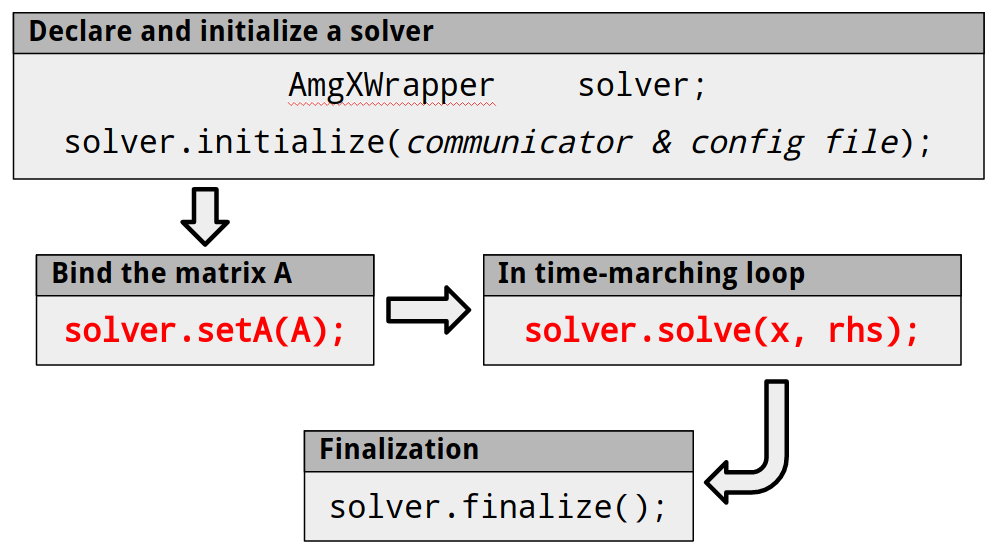
\includegraphics[width=0.6\linewidth]{amgxwrapper.png}
    \caption{Usage of AmgXWrapper in legacy PETSc applications}
    \label{fig:amgxwrapper}
\end{figure}
The configuration of the solvers can be done at runtime, like how PETSc handles those third-party solver providers.

Besides serving as a translation layer, AmgXWrapper resolves an issue when CPUs and GPUs are both used in the calculation.
Commonly, HPC clusters have much more CPU cores than GPUs.
So CFD practitioners usually favor using all CPU cores and GPUs for computing.
However, most multi-GPU libraries were not developed for this use case, including AmgX.
They expect users to use the same number for MPI processes and GPUs.
AmgXWrapper provides a matrix consolidation mechanism for use cases when CPU cores and MPI processes are greater than available GPUs.
For example, most GPUs nowadays do not have enough memory to host a whole 3D CFD problem, so users may choose to use CPUs for solving forcing and velocity systems as they are not performance bottlenecks.
They only use GPUs for pressure solvers to save GPU memory usage.
Therefore, it is natural for these users to use as many CPUs for forcing and velocity as possible, and domain decomposition is done using the same number of MPI processes on CPUs.
When calling pressure solvers on GPUs, the number of subdomains does not match the number of GPUs, and this is when the matrix consolidation layer comes into play, as shown in figure \ref{fig:amgxwrapper-consolidation}.
\begin{figure}[hbt!]
    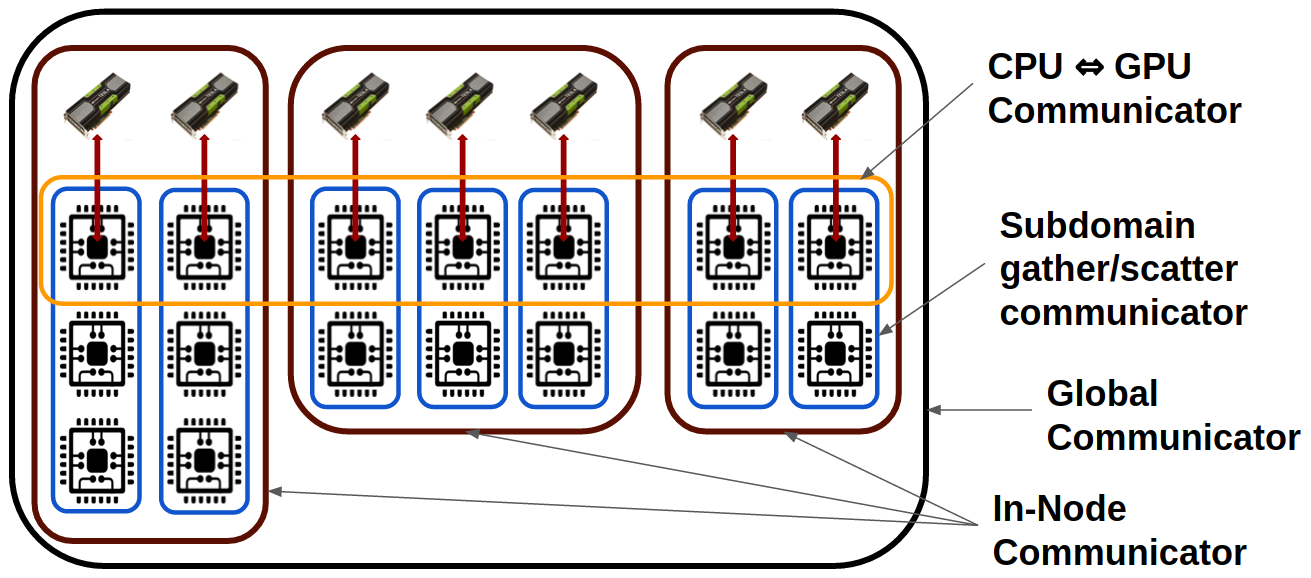
\includegraphics[width=0.6\linewidth]{amgxwrapper-consolidation.png}
    \caption{Graphic illustration of the consolidation layer in AmgXWrapper}
    \label{fig:amgxwrapper-consolidation}
\end{figure}
If without such a consolidation layer, several MPI processes would share one GPU, causing resource competition.

We will show the effect of the consolidation layer together with other performance benchmarks in section \ref{sec:petibm-perf}.
% vim:ft=tex